
\documentclass[crop, tikz, border=0pt]{standalone}
\usetikzlibrary{matrix}
\usetikzlibrary{patterns}
\usepackage{varwidth}
\usepackage{amsmath}
\usepackage{amssymb}
\usepackage{color}

\begin{document}
\color{white}
\definecolor{red}{HTML}{fd5000}
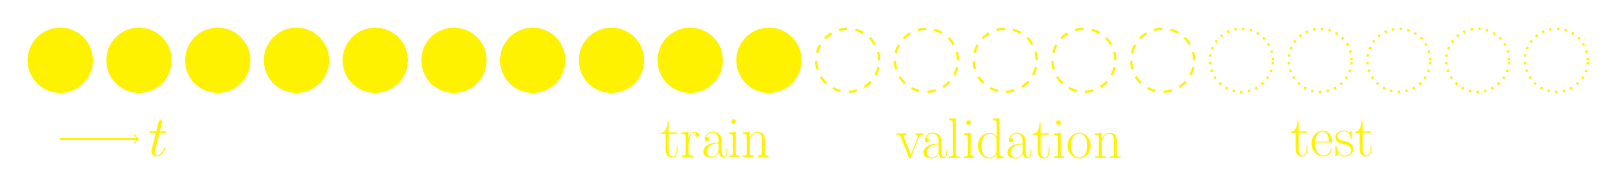
\begin{tikzpicture}[draw=red]
%\tikzset{rectangle node/.style = {rectangle, inner sep=1pt, draw, fill=white}}
\tikzset{edge/.style = {->,> = latex, line width=.5 pt}}

\draw[->, color=yellow] (-5., -.5) --  ++(1, 0) node[right] {\huge $t$} ;
   
\foreach \x in {-5, -4, -3, -2, -1, 0, 1, 2, 3, 4}
   {\draw[thick, fill=yellow, color=yellow]  (\x, .5) circle (.4);}

\foreach \x in {5, 6, 7, 8, 9}
{\draw[thick, dashed, color=yellow]  (\x, .5) circle (.4);}

\foreach \x in {10, 11, 12, 13, 14}
{\draw[thick, dotted, color=yellow]  (\x, .5) circle (.4);}

\node[right, color=yellow, align=left] at (2.5, -.5) {\huge train};
\node[right, color=yellow, align=left] at (5.5, -.5) {\huge validation};   
\node[right, color=yellow, align=left] at (10.5, -.5) {\huge test};  
    
\end{tikzpicture}
\end{document}